% !TeX root = main.tex
\chapter{Methodology}
\label{sec:meth}\label{sec:meth-overview}

\Gls{tls} requires models that separate individual lines reliably while learning from a few annotated pages. Existing methods follow two paradigms (Section~\ref{sec:related-supervised}): semantic segmentation predicts which pixels belong to text lines and separates the lines afterwards, whereas instance segmentation detects every line as an object. To compare both paradigms under the same conditions, this thesis builds two pipelines of each type (Table~\ref{tab:pipelines}): a U-Net with projection cuts and a center-line model for semantic segmentation (Section~\ref{sec:meth-segmentation}), and RT-DETR with a \gls{bbox} U-Net and Mask R-CNN for instance segmentation (Section~\ref{sec:meth-detection}). The U-Net and both detectors are built on the same encoder families, so that the encoder architecture and its initialization can be varied independently of the pipeline (Section~\ref{sec:backbones}). Finally, Section~\ref{sec:shot-sampling} describes the strategies that select the few annotated training pages.

\begin{table}[htbp]
    \centering
    \caption{Evaluated pipelines and how each yields individual text lines.}
    \label{tab:pipelines}
    \small
    \setlength{\tabcolsep}{4pt}
    \begin{tabularx}{\textwidth}{@{}>{\raggedright\arraybackslash}p{2.9cm}>{\raggedright\arraybackslash}p{3.4cm}>{\raggedright\arraybackslash}X>{\raggedright\arraybackslash}p{1.3cm}@{}}
        \toprule
        Pipeline & First stage & Individual lines & Section \\
        \midrule
        \multicolumn{4}{@{}l}{\emph{Semantic segmentation}} \\
        U-Net & U-Net: text line mask of the page & Projection cuts or seams split the mask & \ref{sec:semantic-postprocessing} \\
        Center-line model & U-Net: center lines, line ends, vertical extent & Bands or box for the BBox U-Net (ink masks) & \ref{sec:rq3-center-line} \\
        \midrule
        \multicolumn{4}{@{}l}{\emph{Instance segmentation}} \\
        RT-DETR + BBox U-Net & RT-DETR: one box per line & BBox U-Net in each box & \ref{sec:two-stage-method} \\
        Mask R-CNN & Mask R-CNN: one box and \glsentryshort{roi} mask per line & \glsentryshort{roi} mask, or BBox U-Net in each box & \ref{sec:mask-rcnn-method} \\
        \bottomrule
    \end{tabularx}
\end{table}

\section{Semantic Segmentation}
\label{sec:meth-segmentation}\label{sec:tls-methods}\label{sec:rq3-center-line}

In this type, a U-Net segments the complete page at the pixel level: either the text pixels of the lines as a binary text line mask, or the center line of every line together with its vertical extent. A postprocessing step then extracts the individual lines. In the U-Net pipeline, rules split the mask into lines (Section~\ref{sec:semantic-postprocessing}); in the center-line model, the center lines are grouped and the pixels are assigned to them, using the predicted geometry to separate neighboring lines (Section~\ref{sec:rq3-center-line}). They rely on the encoders described in Section~\ref{sec:backbones}.

\textbf{U-Net with Projection Cuts}\label{sec:semantic-postprocessing} predicts a single text line probability map, which a postprocessing step splits into line instances (Algorithm~\ref{alg:semantic-postprocessing}). First, the map is binarized, and small components are removed. For each remaining component, the row-wise pixel sum forms a horizontal projection, in which peaks mark candidate line centers and a sufficiently deep valley between two peaks marks a cut position. For binary line masks, the baseline prediction of ARU-Net~\cite{gruning2019arunet} is binarized with Otsu's method~\cite{otsu1979threshold}, thinned, and combined with the mask, and the lines are separated along minimum-energy seams through background gaps. For PAGE XML, morphological closing first joins fragmented characters and words. The lines are then separated by straight horizontal cuts and exported as PAGE XML polygons. Figure~\ref{fig:semantic-example} illustrates the steps of Algorithm~\ref{alg:semantic-postprocessing} on a U-DIADS-TL test page: small components such as an isolated marginal letter are removed, and lines that touch in the mask are separated by cuts.

\begin{algorithm}[htbp]
    \small
    \caption{Ground-truth-format-specific postprocessing of a semantic text line probability map}
    \label{alg:semantic-postprocessing}
    \KwIn{Probability map \(P\), page image \(I\), ground-truth representation \(GT\), and main text-region mask \(R\), when available}
    \KwOut{Individual text line components}

    \(M \leftarrow\) binarize \(P\) and remove small foreground components\;

    \eIf{\(GT=\text{binary mask}\)}{
        \(B \leftarrow\) apply Otsu thresholding to the ARU-Net baseline prediction for \(I\)\;
        Thin \(B\), combine it with \(M\), and remove small components\;
        \(C \leftarrow\) minimum-energy seam\;
    }{
        Join character and word fragments using morphological closing\;
        \(C \leftarrow\) straight horizontal cut\;
    }

    Find projection peaks and valleys in each connected component of \(M\)\;
    Separate merged lines through accepted valleys using \(C\)\;
    Remove small fragments created by the cuts\;

    \eIf{\(GT=\text{binary mask}\)}{
        \Return{the connected components of \(M\) as text line instances}\;
    }{
        Clip \(M\) to \(R\)\;
        Discard components that are too small, too short, or insufficiently wide\;
        Convert the remaining components to polygons and baselines in PAGE XML\;
        \Return{the PAGE XML text line polygons}\;
    }
\end{algorithm}

\begin{figure}[htbp]
    \centering
    \begin{subfigure}[t]{0.24\linewidth}\centering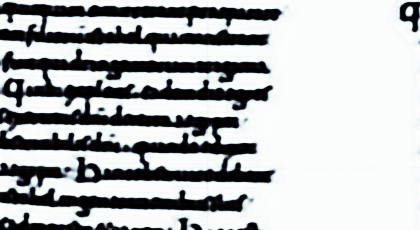
\includegraphics[width=\linewidth]{graphics/unetpp_a_prob.png}\caption{U-Net probability.}\end{subfigure}\hfill
    \begin{subfigure}[t]{0.24\linewidth}\centering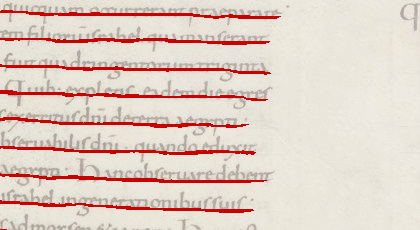
\includegraphics[width=\linewidth]{graphics/unetpp_b_baseline.png}\caption{ARU-Net baselines.}\end{subfigure}\hfill
    \begin{subfigure}[t]{0.24\linewidth}\centering
\includegraphics[width=\linewidth]{graphics/unetpp_c_fused.png}\caption{Fused mask.}\end{subfigure}\hfill
    \begin{subfigure}[t]{0.24\linewidth}\centering
\includegraphics[width=\linewidth]{graphics/unetpp_d_instances.png}\caption{Line instances.}\end{subfigure}
    \caption{U-Net postprocessing for binary line masks (U-DIADS-TL Latin2, test page 076): (a) line probability, (b) ARU-Net baselines~\cite{gruning2019arunet}, (c) thresholded mask with baselines, removed components (red), and cuts (blue), (d) line instances. Generated from U-DIADS-TL~\cite{Zottin_2025_FEST}.}
    \label{fig:semantic-example}
\end{figure}



\textbf{Center-Line Model} keeps the U-Net architecture of Section~\ref{sec:semantic-postprocessing}, but instead of a binary text line mask it predicts the center line of every text line and its distances to the upper and lower line boundary, and it assigns the ink pixels to the nearest center line rather than constructing a polygon. Line instances are thus reconstructed from the center lines, without requiring \glspl{bbox}; missed or incorrectly grouped centers can still merge or split lines. Figure~\ref{fig:center-line-method} illustrates the predicted maps and the decoding, and Table~\ref{tab:rq3-center-line-settings} in Section~\ref{sec:training-setup} lists the settings. For datasets whose binary-mask \gls{gt} marks ink pixels rather than line regions, the center-line model serves as a line detector for the BBox U-Net (Section~\ref{sec:training-center-line}).

\begin{figure}[htbp]
    \centering
    \begin{subfigure}[t]{0.49\linewidth}\centering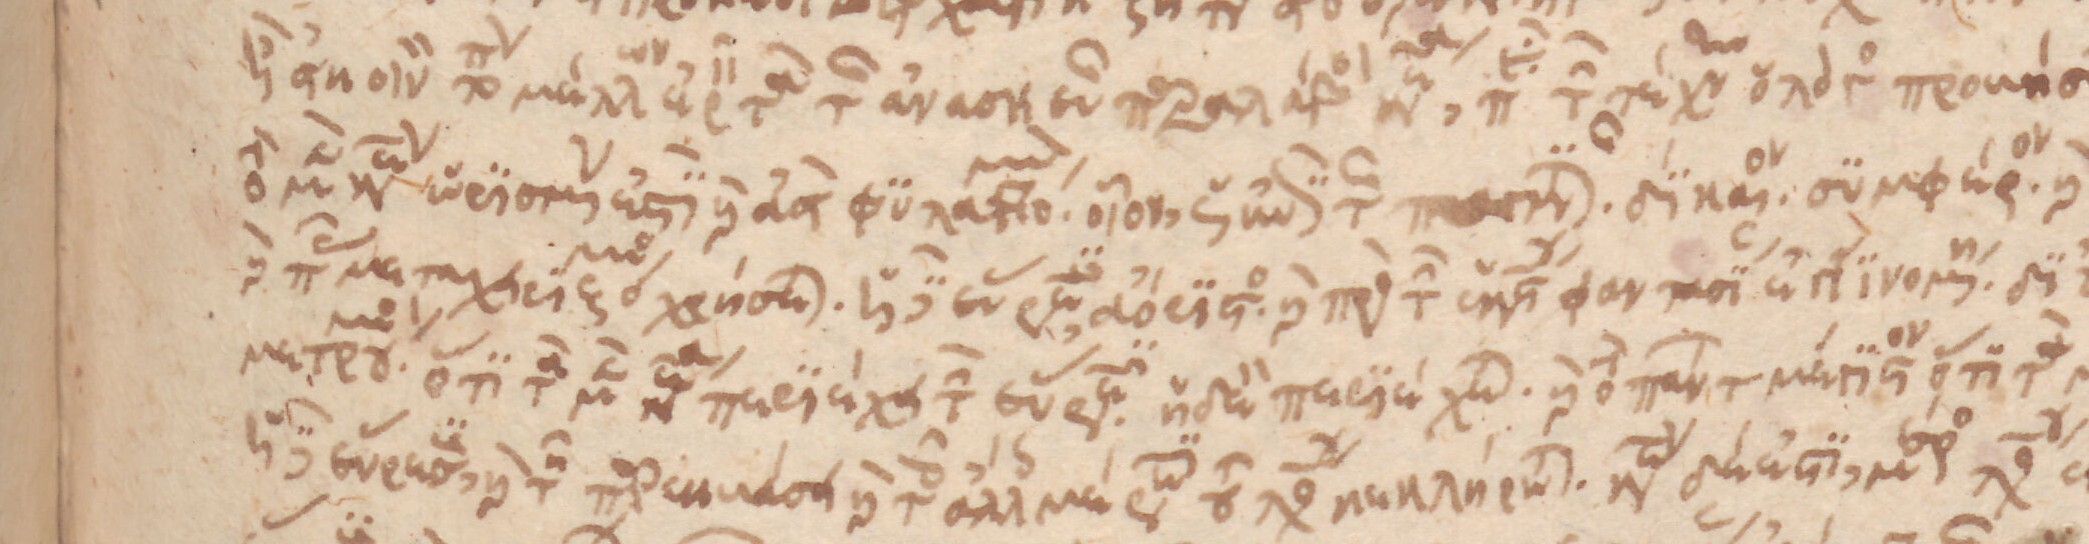
\includegraphics[width=\linewidth]{graphics/cl_method_a.jpg}\caption{Input crop.}\label{fig:center-line-method-a}\end{subfigure}\hfill
    \begin{subfigure}[t]{0.49\linewidth}\centering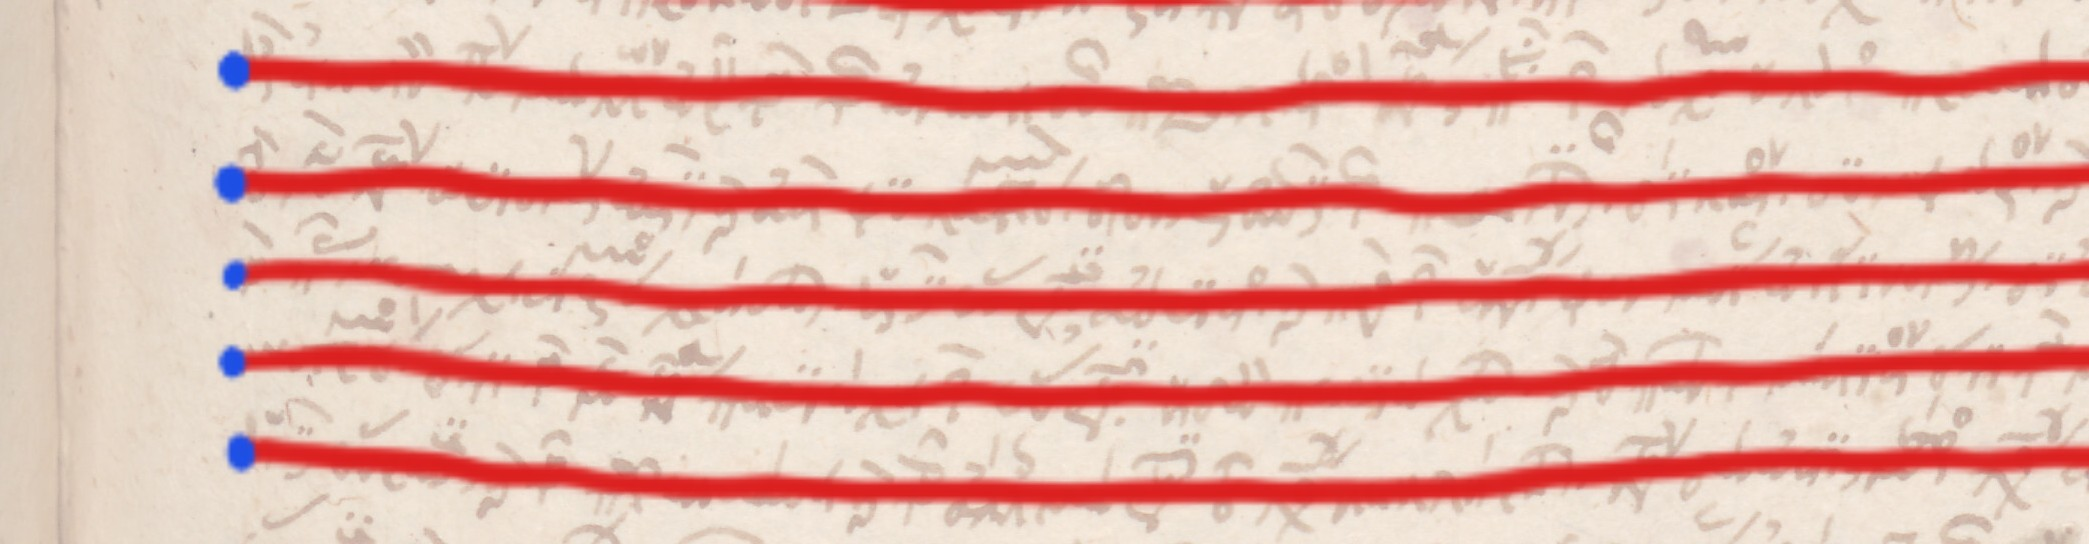
\includegraphics[width=\linewidth]{graphics/cl_method_b.jpg}\caption{Center map (red) and line-end map (blue).}\label{fig:center-line-method-b}\end{subfigure}

    \medskip
    \begin{subfigure}[t]{0.49\linewidth}\centering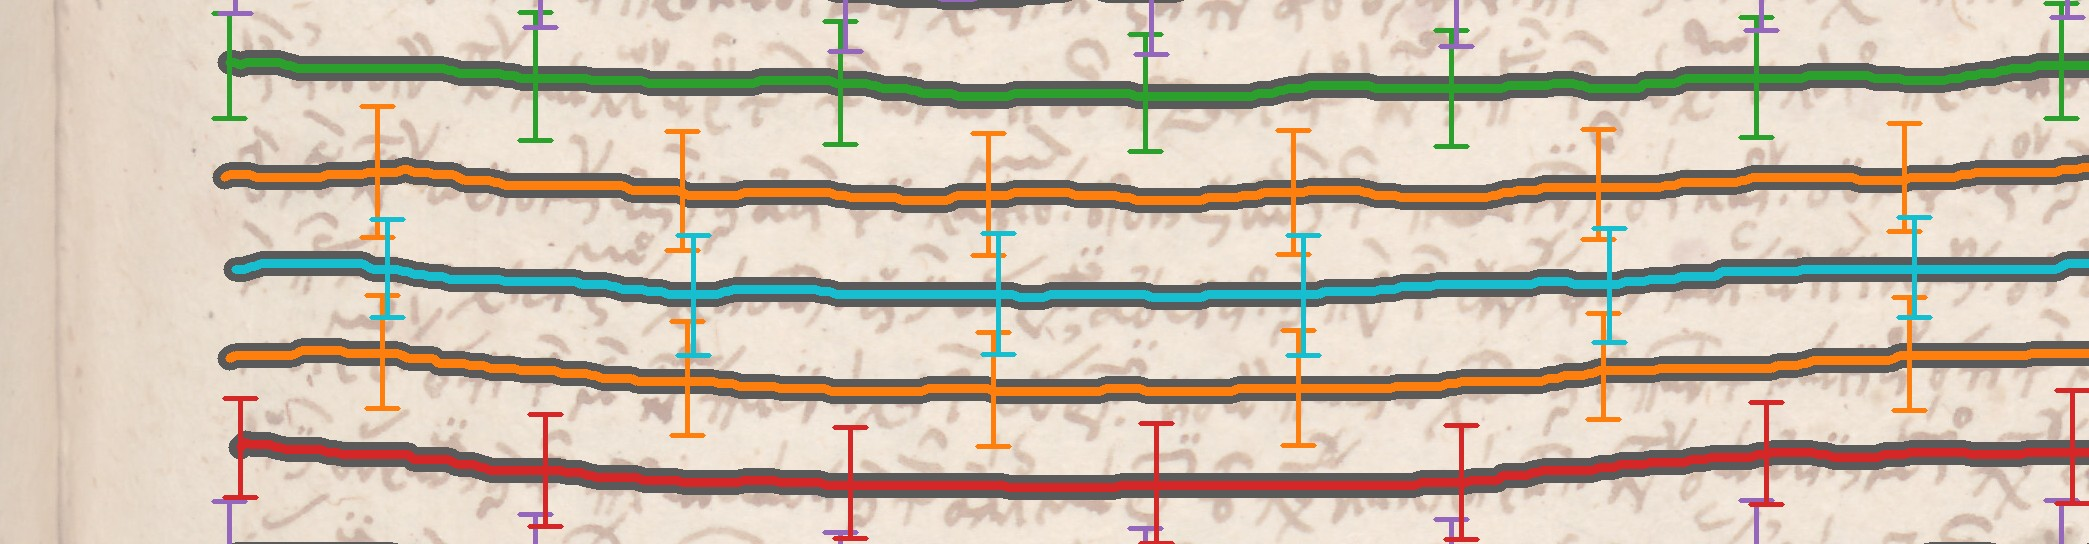
\includegraphics[width=\linewidth]{graphics/cl_method_c.jpg}\caption{Fragments (gray) joined into center lines; vertical bars show the predicted distances to the upper and lower line boundary.}\label{fig:center-line-method-c}\end{subfigure}\hfill
    \begin{subfigure}[t]{0.49\linewidth}\centering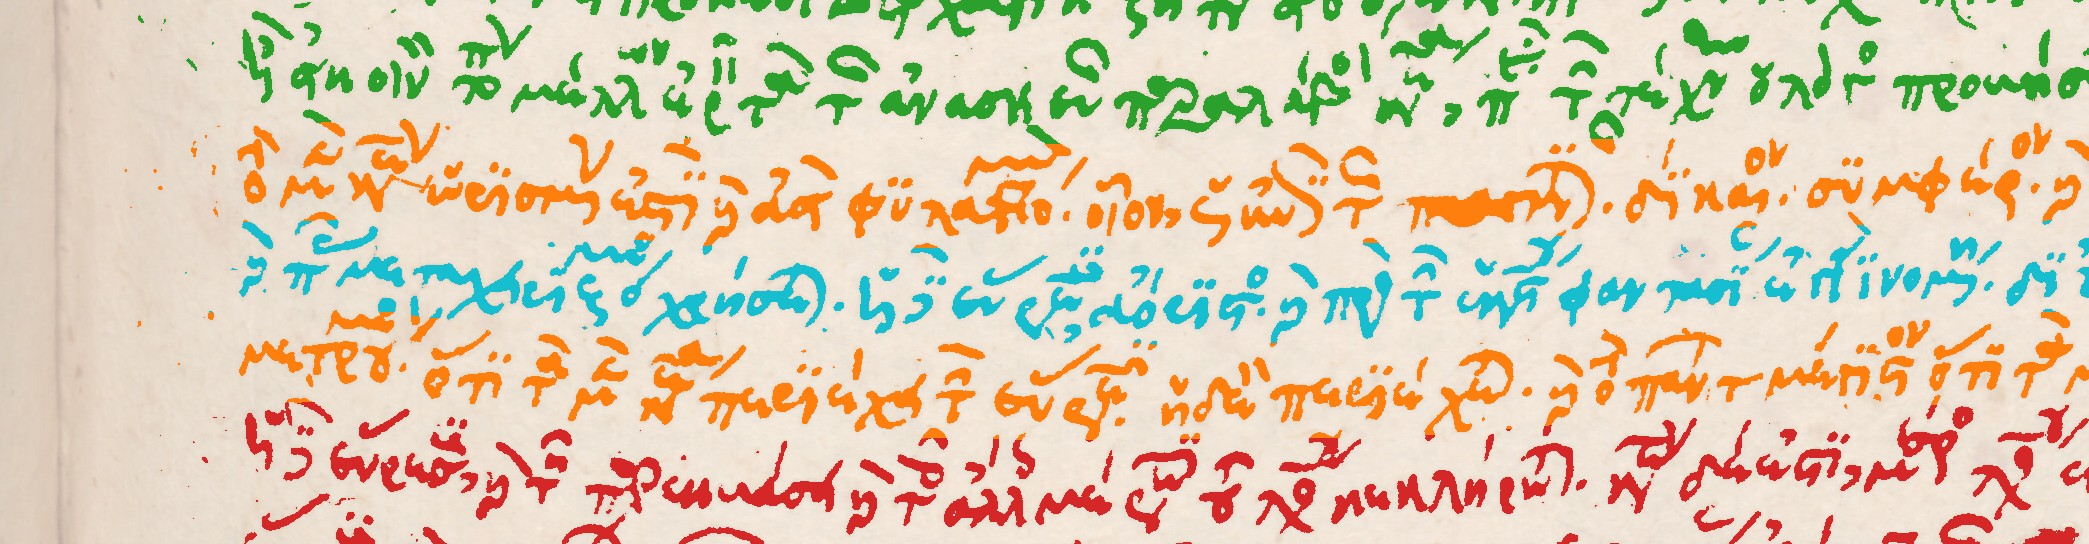
\includegraphics[width=\linewidth]{graphics/cl_method_d.jpg}\caption{Ink pixels assigned to the nearest center line.}\label{fig:center-line-method-d}\end{subfigure}
    \caption{Center-line model on a Phil.\ gr.\ 130 development page (trained on three ONB Cod.\ Syr.\ 1 pages). Generated from Phil.\ gr.\ 130~\cite{SindlevAndersen2026PhilGrGT}.}
    \label{fig:center-line-method}
\end{figure}

The U-Net predicts four maps: the probability of the line center, the probability of a line end, and the distances from the center line to the upper and to the lower boundary of the line polygon. The targets are derived for every pixel column from the annotated polygons. The center is the midpoint between the upper and lower polygon boundaries, and both distances are measured from it. To make the line size comparable across pages, each training page is rescaled so that its median line thickness equals \(T_0=24\) pixels, and then by a random factor \(2^{z}\) with \(z\sim\mathcal{N}(0,0.6^2)\). The loss sums binary cross-entropy and Dice terms for the center map and, with weight 0.5, for the end map, and adds a smooth \(L_1\) term for the two distances on center pixels.

At inference, a page is first processed with its long side scaled. The median predicted line thickness on center pixels then determines a second scale, at which the lines have thickness \(T_0\), and the page is processed again. The center map, reduced by half of the end map, is thresholded and split into connected fragments, and each fragment is represented by its mean row per pixel column. These fragments are joined from left to right into lines when the horizontal gap is small and the vertical offset from the extrapolated line is small relative to the line pitch \(p\). Here, \(p\) is the median vertical distance between horizontally overlapping neighboring fragments of the page. Lines shorter than \(0.5\,p\) are discarded. Finally, every pixel is assigned to its nearest center line if their distance does not exceed \(p\). On DIVA-HisDB, the line region is instead the band between the predicted upper and lower distances inside this cell. Ink components that touch the band are added to it, and components that reach into a neighboring line are split along the minimum-ink seam between the two center lines. The instances are exported as PAGE XML elements.

\FloatBarrier

\section{Instance Segmentation}
\label{sec:meth-detection}

In this type, every text line is treated as an object. A detector first predicts one \gls{bbox} per text line, and a second stage then decides which pixels inside each box belong to the line.

\subsection{Line Detection}
\label{sec:detectors}

RT-DETR only predicts boxes, whereas Mask R-CNN additionally predicts a coarse mask for every box. Figure~\ref{fig:two-stage-method} shows how both detectors are combined with the second stage.

\begin{figure}[htbp]
    \centering
    % Simple schematic of the instance segmentation pipelines (RT-DETR and Mask R-CNN) with a shared encoder.
\begingroup
% Shared visual language for the three segmentation-method diagrams.
\tikzset{
    box/.style={draw, rounded corners=2pt, align=center, font=\small,
        text width=44mm, minimum height=9mm, inner sep=4pt, line width=0.5pt},
    process/.style={box, fill=gray!7},
    model/.style={box, very thick, fill=blue!5},
    output/.style={box, dashed},
    supervision/.style={box, densely dashed, fill=gray!7},
    link/.style={->, semithick},
    traininglink/.style={link, densely dashed}
}

\usetikzlibrary{calc}
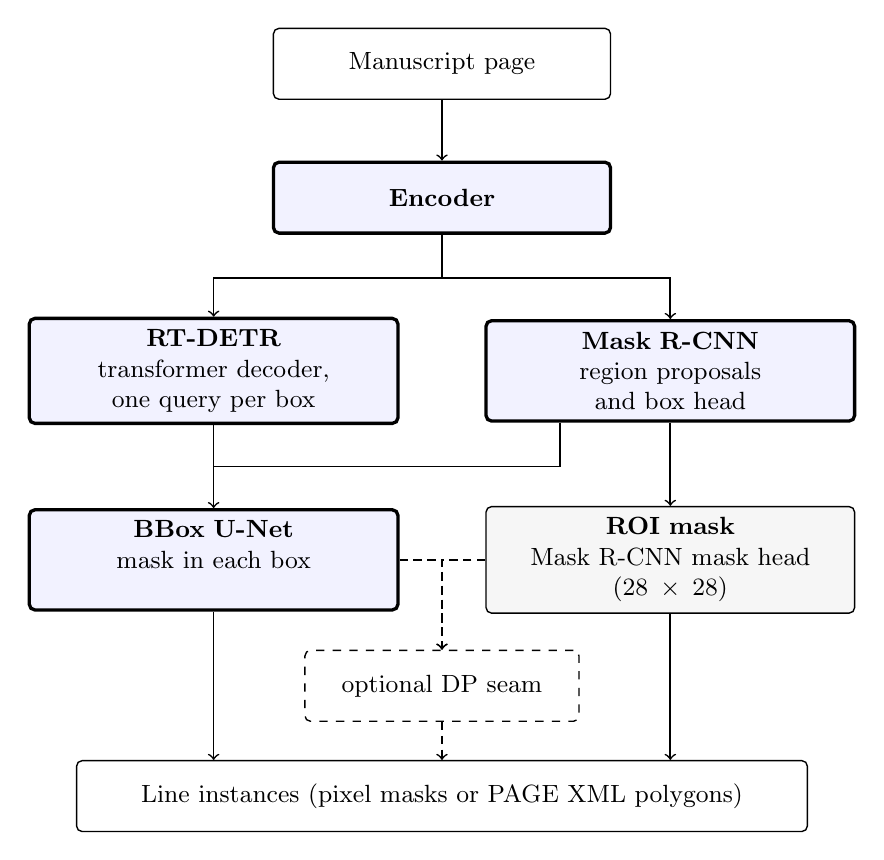
\begin{tikzpicture}
    \node[box, text width=40mm] (page) at (0,0) {Manuscript page};
    \node[model, text width=40mm] (enc) at (0,-1.7) {\textbf{Encoder}};
    \node[model, text width=44mm] (rtdetr) at (-2.9,-3.9) {\textbf{RT-DETR}\\transformer decoder,\\one query per box};
    \node[model, text width=44mm] (mrcnn) at (2.9,-3.9) {\textbf{Mask R-CNN}\\region proposals\\and box head};
    \node[model, text width=44mm] (crop) at (-2.9,-6.3) {\textbf{BBox U-Net}\\mask in each box\\\phantom{x}};
    \node[process, text width=44mm] (roi) at (2.9,-6.3) {\textbf{ROI mask}\\Mask R-CNN mask head\\(\(28\times28\))};
    \node[output, text width=32mm] (seam) at (0,-7.9) {optional DP seam};
    \node[box, text width=90mm] (lines) at (0,-9.3) {Line instances (pixel masks or PAGE XML polygons)};
    \draw[link] (page) -- (enc);
    % fork from the shared encoder to both detectors
    \coordinate (fork) at ($(enc.south)+(0,-0.55)$);
    \draw[semithick] (enc.south) -- (fork);
    \draw[link] (fork) -| (rtdetr.north);
    \draw[link] (fork) -| (mrcnn.north);
    \draw[link] (rtdetr.south) -- (rtdetr.south |- crop.north);
    % Mask R-CNN boxes join the RT-DETR -> BBox U-Net arrow
    \coordinate (mstart) at ($(mrcnn.south)+(-1.4,0)$);
    \coordinate (join) at ($(rtdetr.south)!0.5!(rtdetr.south |- crop.north)$);
    \draw[semithick] (mstart) |- (join);
    \draw[link] (mrcnn.south) -- (mrcnn.south |- roi.north);
    \draw[traininglink] (crop.east) -| (seam.north);
    \draw[traininglink] (roi.west) -| (seam.north);
    \draw[traininglink] (seam.south) -- (lines.north);
    \draw[link] (crop.south) -- (crop.south |- lines.north);
    \draw[link] (roi.south) -- (roi.south |- lines.north);
\end{tikzpicture}
\endgroup

    \caption{Instance segmentation pipelines with a shared encoder. The BBox U-Net segments the boxes of either detector; the optional \gls{dp} seam (dashed) exports the mask of each box.}
    \label{fig:two-stage-method}\label{fig:mask-rcnn-architecture}
\end{figure}

\paragraph{RT-DETR with BBox Segmentation}\label{sec:two-stage-method} separates the localization of a line from the prediction of its boundary. First, an RT-DETR detector~\cite{Zhao_2024_CVPR} predicts one \gls{bbox} per text line on the complete page. Its confidence threshold is selected on the validation split, and duplicate detections are removed. The training settings of the detector and the BBox U-Net are given in Section~\ref{sec:training-two-stage}.

\paragraph{Mask R-CNN}\label{sec:mask-rcnn-method}~\cite{he2017maskrcnn} treats every text line as a separate object of a single foreground class. First, a region proposal network generates candidate boxes. RoIAlign then extracts aligned features for each proposal, from which parallel heads classify the proposal, refine its box, and predict its mask. The mask head predicts a \(28\times28\) mask from \(14\times14\) RoIAlign features, and this mask is resized to the size of the box at inference. Each accepted proposal has its own mask, allowing neighboring or overlapping lines to be represented separately; this does not guarantee that each proposal corresponds to exactly one line. Its training settings are given in Section~\ref{sec:training-mask-rcnn}.

At inference, the detections are processed in descending confidence order, and their masks are restored to the original page resolution. The confidence threshold is selected on the validation split by minimizing the absolute error of the predicted line count, and the mask threshold is fixed at 0.5. Each mask is clipped to the annotated main text region, and its largest contour is exported as a PAGE XML polygon, while the lower edge of its bounding rectangle defines the baseline.

\subsection{Line Reconstruction}
\label{sec:crop-unet}\label{sec:integration}\label{sec:boundary-heads}

The second stage determines which pixels inside each detected box belong to the line. Mask R-CNN provides its native \gls{roi} mask, whereas the BBox U-Net segments every box separately and can be applied to the boxes of both detectors. Every accepted box yields one candidate line, and the page-level output is assembled in descending detection confidence by rules that depend on the \gls{gt} format. For binary-mask \gls{gt}, the masks are pasted into an empty page-sized instance map, and pixels that are already assigned are not overwritten. For PAGE XML format, the largest contour of each mask becomes the line polygon, and the baseline is derived from its lower boundary. As a consequence, parts of a line that are disconnected in the mask might be discarded.

Figure~\ref{fig:two-stage-example} illustrates these rules on one page, where the region and width filters reduce 289 raw detections to 33.

\begin{figure}[htbp]
    \centering
    \begin{subfigure}[t]{0.49\linewidth}\centering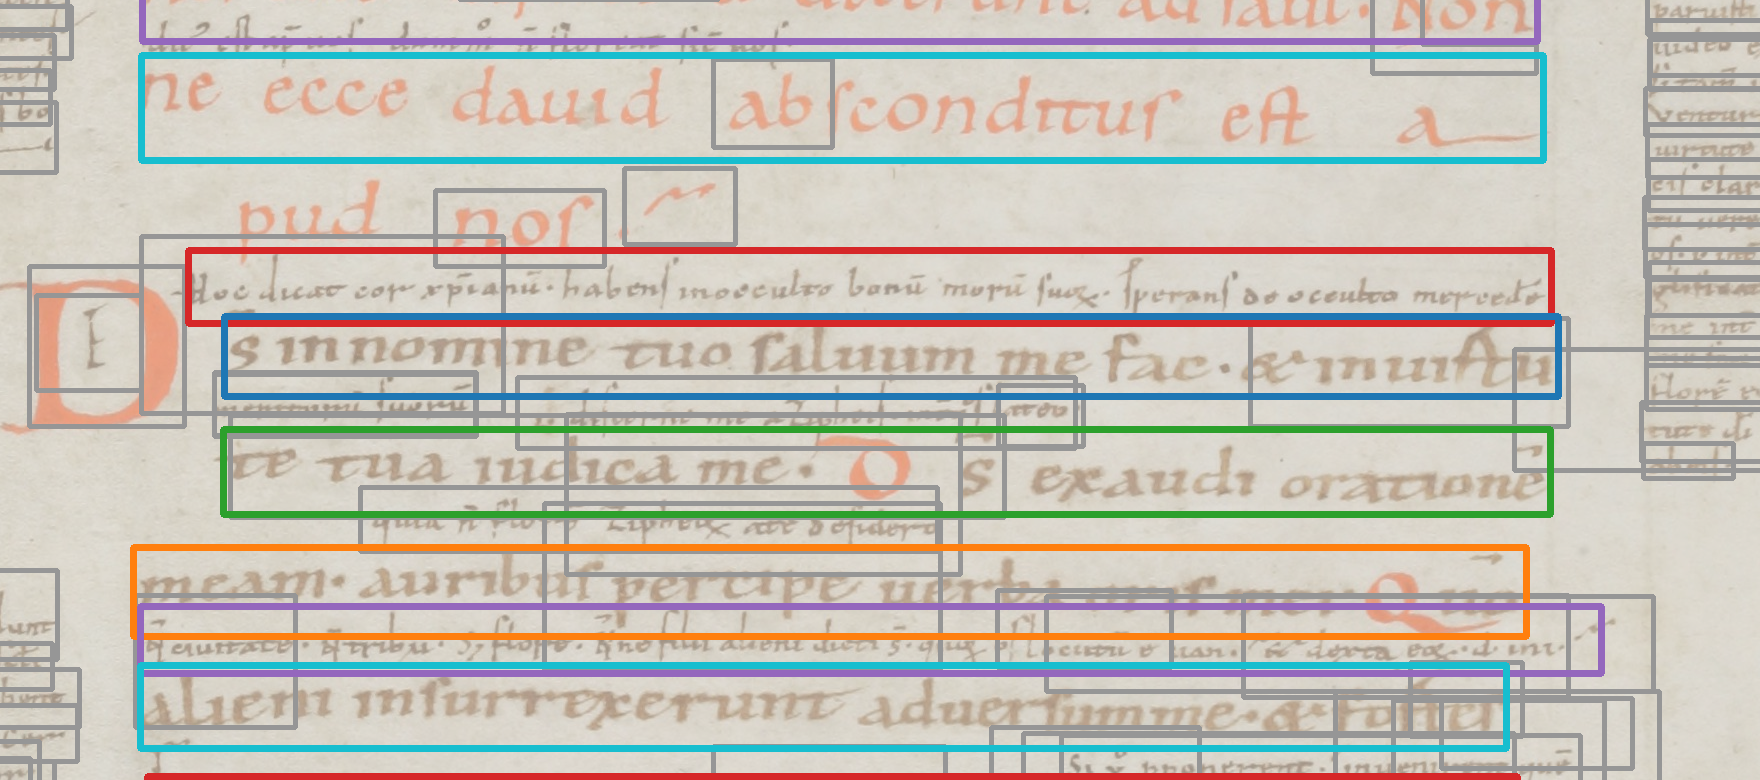
\includegraphics[width=\linewidth]{graphics/twostage_cs18_096_boxes.png}\caption{RT-DETR boxes, kept (colored) and discarded by the filters (gray).}\label{fig:two-stage-example-boxes}\end{subfigure}\hfill
    \begin{subfigure}[t]{0.49\linewidth}\centering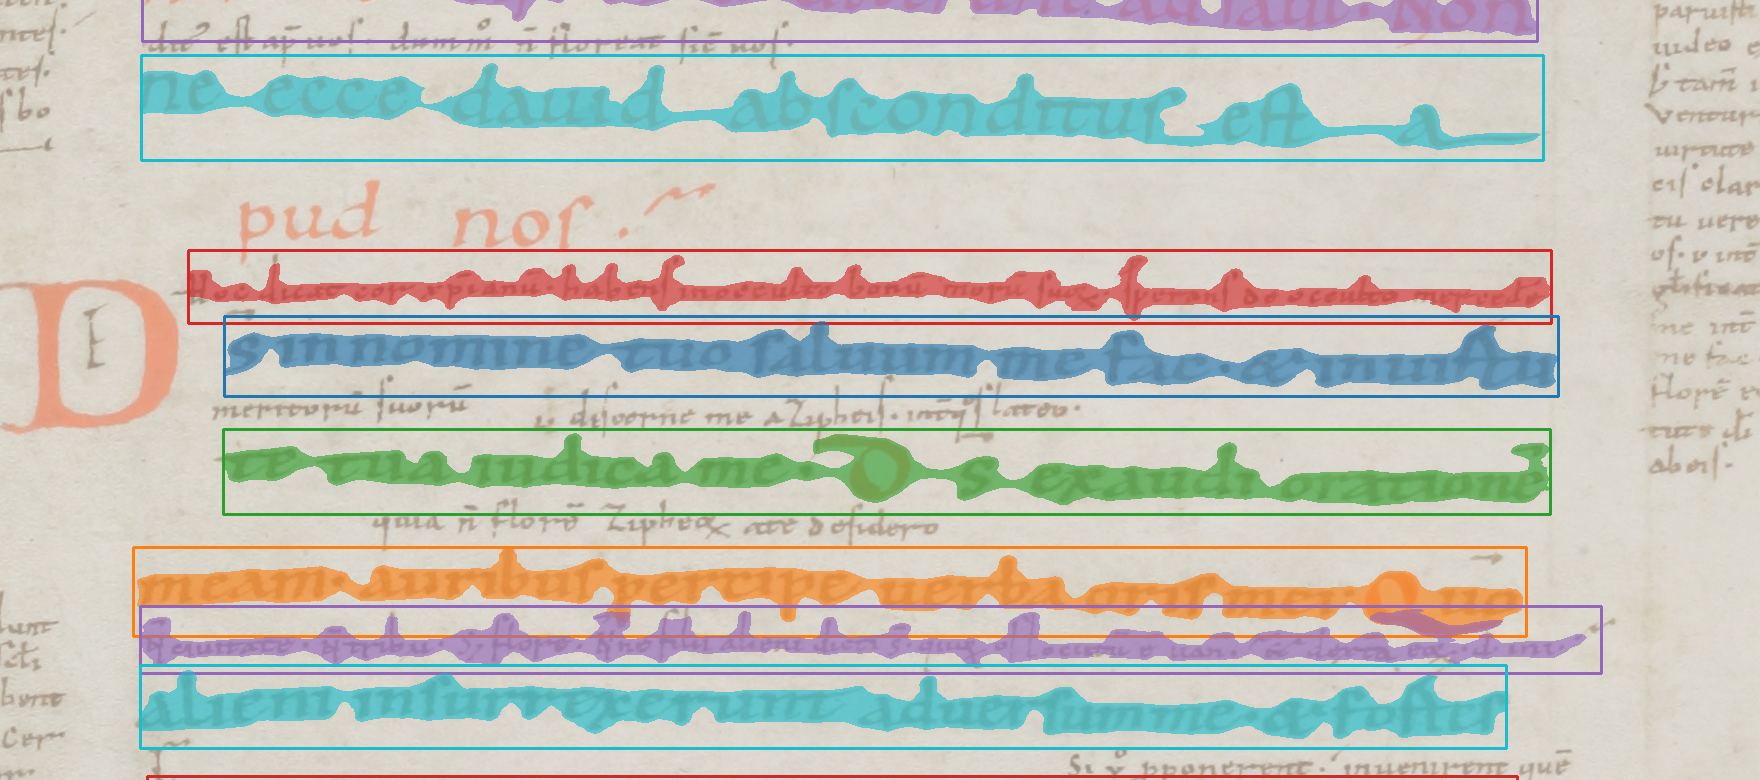
\includegraphics[width=\linewidth]{graphics/twostage_cs18_096_masks.png}\caption{BBox U-Net masks inside the kept RT-DETR boxes.}\label{fig:two-stage-example-masks}\end{subfigure}\\[4pt]
    \begin{subfigure}[t]{0.49\linewidth}\centering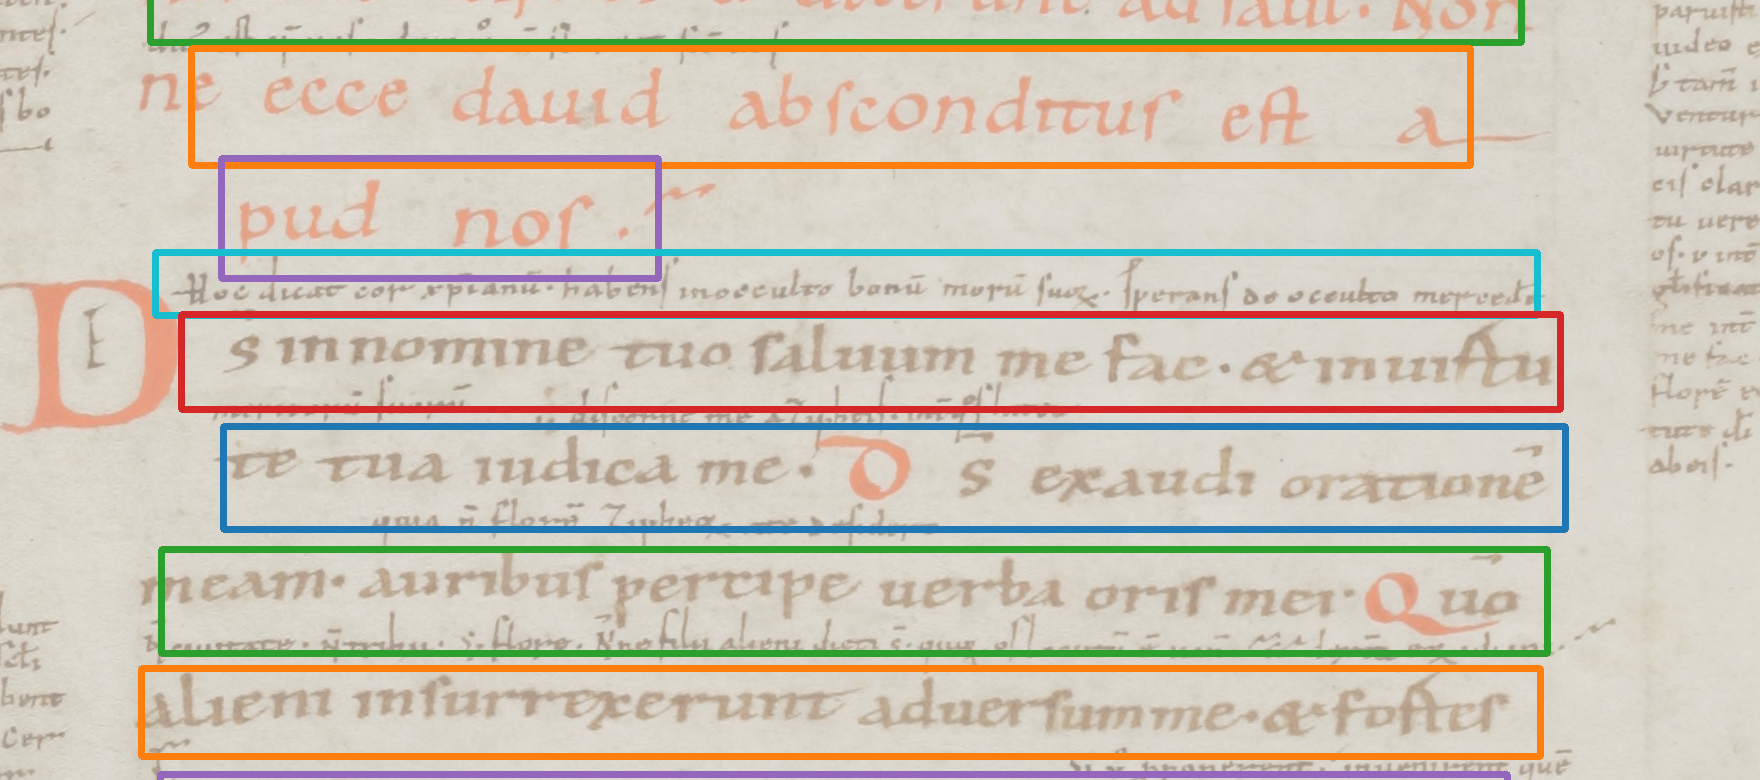
\includegraphics[width=\linewidth]{graphics/maskrcnn_cs18_096_boxes.png}\caption{Mask R-CNN boxes of the exported detections.}\label{fig:two-stage-example-mrcnn-boxes}\end{subfigure}\hfill
    \begin{subfigure}[t]{0.49\linewidth}\centering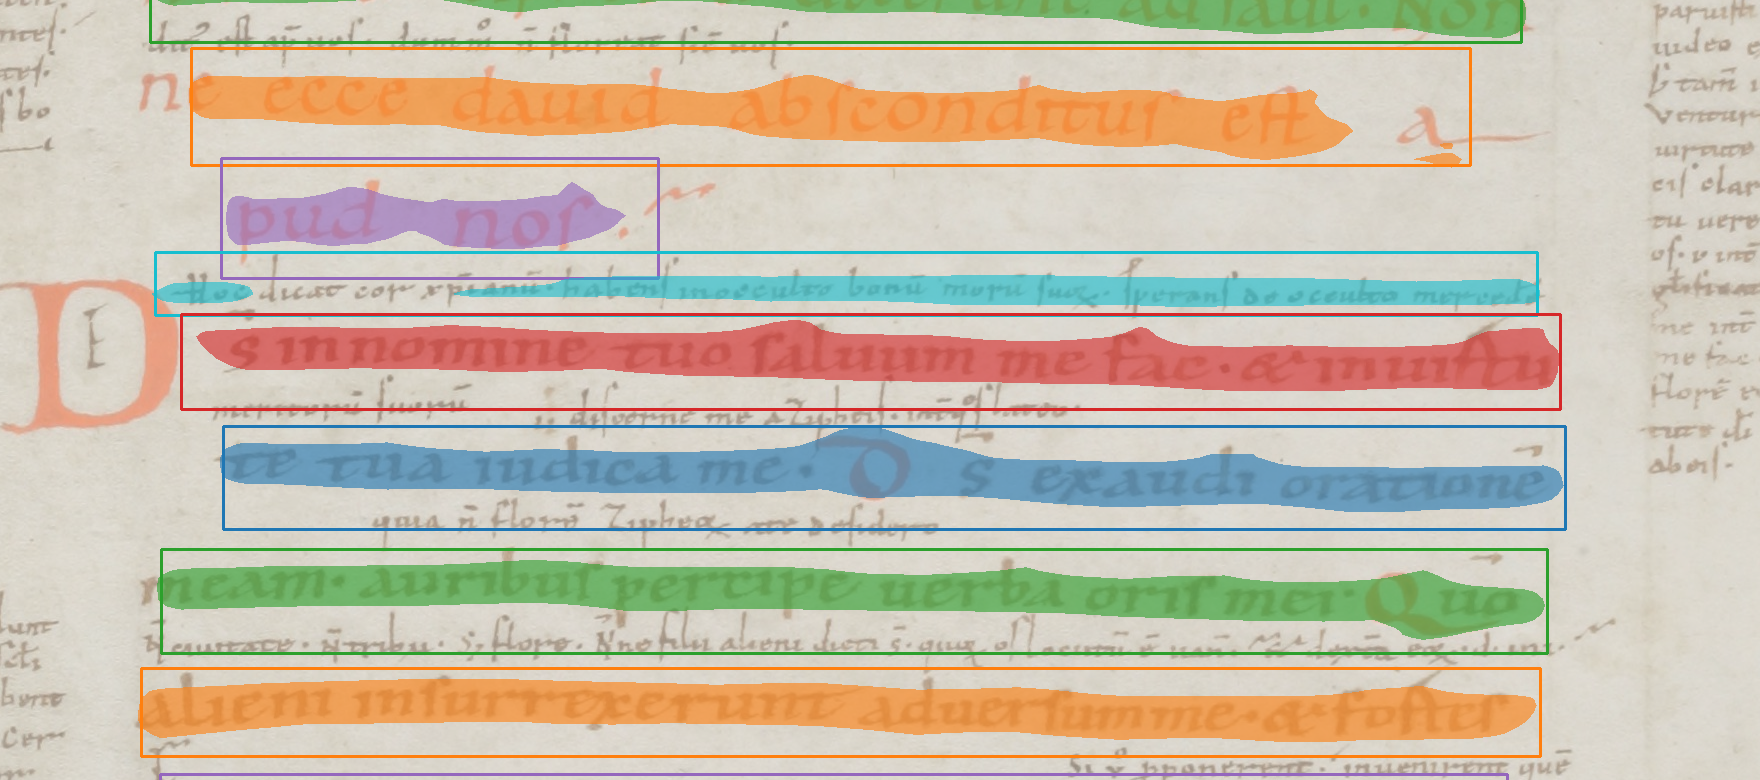
\includegraphics[width=\linewidth]{graphics/maskrcnn_cs18_096_masks.png}\caption{Mask R-CNN \glsentryshort{roi} masks inside these boxes.}\label{fig:two-stage-example-mrcnn-masks}\end{subfigure}
    \caption{RT-DETR + BBox U-Net (a, b) and Mask R-CNN (c, d) on a region of CS18 test page 096. Generated from DIVA-HisDB~\cite{diva_hisdb}.}
    \label{fig:two-stage-example}
\end{figure}

\paragraph{BBox U-Net and \gls{roi} Head}\label{sec:crop-roi} predict the mask of each detected line. The BBox U-Net is a U-Net~\cite{DBLP:journals/corr/RonnebergerFB15} with a ResNet-34 encoder that segments each line crop, whereas the \gls{roi} head is the mask branch of Mask R-CNN. The training targets of the BBox U-Net are derived from the \gls{gt}: each PAGE XML polygon, or each component of a binary mask, defines a \gls{bbox}, and the line mask inside this box forms the target. For binary masks, only the selected component is retained. The box is padded to keep some context, and both crop and target are resized to a common elongated input size. In the comparison of detector backbones, the BBox U-Net is kept fixed, so that the differences can be attributed to the detector.

At inference, each retained detection is padded in the same way and segmented independently. The probability map is resized to the native crop size before thresholding, and only its main connected component is kept. For binary-mask datasets, a horizontal morphological closing can additionally join fragmented parts of a line. The binarization threshold (0.5, 0.7, or 0.9) and the closing width (none or 4\% of the crop width) are selected per detector on the validation split by the mean line-level \gls{fm}, in the same way as the detection threshold. For PAGE XML datasets, the detections are restricted to the annotated main text region, overlapping row detections are removed, and a validation-selected width filter discards short detections.

On U-DIADS-TL, however, the coarse \gls{roi} masks do not match the pixel-accurate binary \gls{gt}. For this reason, the \gls{roi} masks are replaced by the BBox U-Net, while Mask R-CNN still supplies the proposals, their scores, and the instance identities. Each accepted box is padded, and the crop is resized to \(1024\times256\) pixels and segmented. The confidence threshold is selected on the validation split by the box F1 score at an \gls{iou} of 0.5, and the padding, the crop-mask threshold, and a minimum instance area are then selected on the validation split by \gls{fm}. Table~\ref{tab:second-stage} compares these masks with the native \gls{roi} masks for the same detections. In this configuration, only the box branch of Mask R-CNN is used at inference, which corresponds to Faster R-CNN~\cite{ren2017fasterrcnn} with a feature pyramid network and RoIAlign~\cite{he2017maskrcnn}. Its weights, however, result from joint training with the mask branch.

To analyze the components of the RT-DETR + BBox U-Net pipeline (Table~\ref{tab:rq1-twostage-components}), the DIVA-HisDB detector boxes are compared with the Task~2 line boxes at \gls{iou} thresholds of 0.5 and 0.75, where \gls{ap} at 0.5 includes detections with a confidence of at least 0.01. The quality of the crop masks is measured by the pixel \gls{iou} with the \gls{gt} polygon inside each \gls{gt} box. In addition, two diagnostic conditions replace either the predicted boxes with \gls{gt} boxes or the masks in matched predicted boxes with clipped \gls{gt} polygons; unmatched predicted boxes keep their crop masks. The page-level outputs use the validation-selected operating points and the DIVA evaluator.

\paragraph{Dynamic-Programming Seam}\label{sec:dp-seam} is an optional postprocessing step for the mask of each box, either the BBox U-Net output of both pipelines or the \gls{roi} mask of Mask R-CNN. It addresses the export of only the largest contour of a crop mask, which discards every part of a line that is disconnected from its largest component, for example at a wide word gap (Figure~\ref{fig:two-stage-example}d). The seam leaves the detections and the masks unchanged and replaces only their export. Instead of the largest contour, it derives a line region that is connected by construction (Algorithm~\ref{alg:dp-seam}). The seam operates on the mask probability map \(P\) of a box, from the BBox U-Net or the \gls{roi} head, averaged over columns of four pixels. In every column, a center row is estimated as the maximum of the vertically smoothed map and interpolated across word gaps. Then, an upper path above and a lower path below the center rows are found by \gls{dp}. Together, the two paths maximize the sum of \(P-t\) over the pixels between them, where \(t\) is the mask threshold, and each path may move by at most \(K\) rows between neighboring columns. For PAGE XML, the region between the paths is exported as the line polygon, whereas for binary masks it is intersected with the thresholded crop mask. Figure~\ref{fig:dp-seam-example} illustrates the steps on a line whose crop mask is split at two word gaps, where the largest contour discards 69\% of the thresholded mask.

\begin{figure}[htbp]
    \centering
    \begin{minipage}[c]{0.66\linewidth}
        \begin{subfigure}[t]{\linewidth}\centering
\includegraphics[width=\linewidth]{graphics/dpseam_a.png}\caption{Largest-contour export: the crop mask is split at two word gaps; the orange part is kept and the red parts are discarded.}\label{fig:dp-seam-example-a}\end{subfigure}\\[6pt]
        \begin{subfigure}[t]{\linewidth}\centering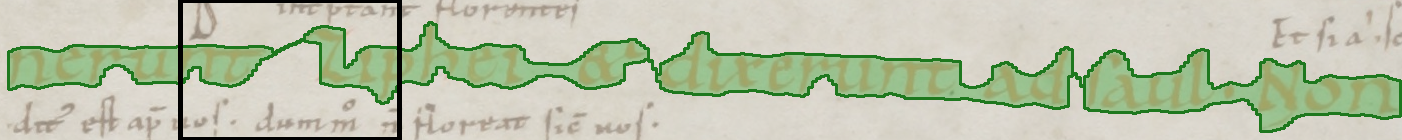
\includegraphics[width=\linewidth]{graphics/dpseam_c.png}\caption{Seam export: the region between the two paths (green) covers the complete line.}\label{fig:dp-seam-example-c}\end{subfigure}
    \end{minipage}\hfill
    \begin{minipage}[c]{0.3\linewidth}
        \begin{subfigure}[t]{\linewidth}\centering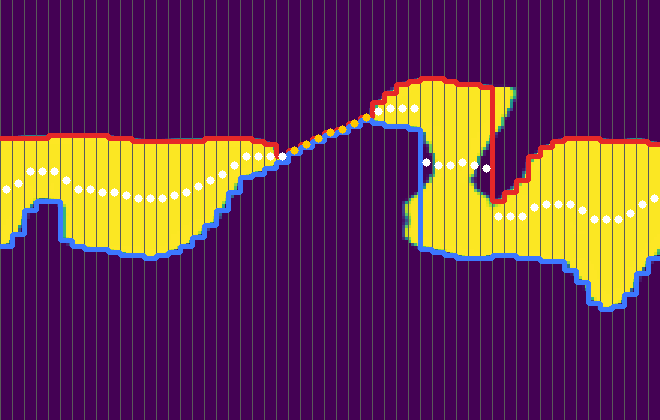
\includegraphics[width=\linewidth]{graphics/dpseam_b.png}\caption{Black window of (a) and (b): probability \(P\), center rows (white; interpolated in orange), and the upper (red) and lower (blue) paths.}\label{fig:dp-seam-example-b}\end{subfigure}
    \end{minipage}
    \caption{\Gls{dp} seam on one detected line of CS18 test page 096. In the word gaps, both paths follow the interpolated center rows and keep the line connected. Generated from DIVA-HisDB~\cite{diva_hisdb}.}
    \label{fig:dp-seam-example}
\end{figure}

\begin{algorithm}[htbp]
    \small
    \caption{\Gls{dp} seam for one detected line}
    \label{alg:dp-seam}
    \KwIn{Crop probability map \(P\), mask threshold \(t\), maximum step \(K\)}
    \KwOut{Line region between an upper and a lower path}
    Average \(P\) over columns of four pixels and keep the columns between the first and the last column whose maximum is at least \(t\)\;
    \(c_x \leftarrow\) row of the maximum of the vertically smoothed \(P\) in column \(x\); interpolate \(c\) in columns whose maximum is below \(t\)\;
    \(u \leftarrow \arg\max_{u} \sum_{x}\sum_{y=u_x}^{c_x} (P_{y,x}-t)\) subject to \(u_x \le c_x\) and \(|u_x-u_{x-1}| \le K\)\;
    \(l \leftarrow \arg\max_{l} \sum_{x}\sum_{y=c_x}^{l_x} (P_{y,x}-t)\) subject to \(l_x \ge c_x\) and \(|l_x-l_{x-1}| \le K\)\;
    \Return{the region between \(u\) and \(l\)}\;
\end{algorithm}

\section{Encoders and Pretraining}
\label{sec:backbones}

The U-Net and both detectors use the same encoders, so that an encoder can be exchanged without changing the rest of a pipeline. The comparison covers three architectures that differ in how they process the page: a convolutional network, a hierarchical transformer, and a plain transformer. Their medium-sized variants have a similar number of parameters, between 21.7M and 27.8M (Table~\ref{tab:backbones}). The two hierarchical encoders output feature maps at four resolutions, which the decoders use directly, whereas the plain transformer outputs a single resolution that is converted into a feature pyramid:
\label{sec:encoder-architectures}
\begin{itemize}
    \item \textbf{ConvNeXt}~\cite{liu2022convnet2020s} is a convolutional network modernized with design elements of \glspl{vit}, such as large kernels and layer normalization. ConvNeXt-Tiny outputs feature maps with 96, 192, 384, and 768 channels at strides of 4, 8, 16, and 32 pixels.
    \item \textbf{PVTv2}~\cite{wang2022pvtv2}, the Pyramid Vision Transformer v2, computes attention over spatially reduced keys and values, so that it can process high-resolution feature maps. PVTv2-B2 outputs feature maps with 64, 128, 320, and 512 channels at the same strides.
    \item \textbf{\gls{vit}}~\cite{dosovitskiy2021imageworth16x16words} splits the page into patches of \(16\times16\) pixels and processes them with global self-attention at a single resolution. ViT-Small outputs one feature map with 384 channels at a stride of 16 pixels, from which transposed convolutions derive maps at strides of 4 and 8 pixels and max-pooling a map at a stride of 32 pixels.
\end{itemize}
Encoder architecture and initialization are varied as two separate factors.

\label{sec:initializations}

The comparison of initializations distinguishes two aspects: generic images versus document images, and pretraining without line annotations versus task-specific line supervision. Five initialization strategies are considered:

\begin{itemize}
    \item \textbf{Random.} The encoder weights are drawn with the default initialization of the respective framework, so that the encoder learns its features only from the few training pages.
    \item \textbf{ImageNet.} The encoder uses weights from supervised image classification on ImageNet~\cite{deng2009imagenet}.
    \item \textbf{DINOv3 (LVD-1689M).} The encoder uses the DINOv3 weights, which are distilled from a large \gls{vit} teacher pretrained with \gls{ssl} on 1.7 billion web images (LVD-1689M)~\cite{dinov3}. These weights exist for ConvNeXt-Tiny and ViT-Small, but not for PVTv2.
    \item \textbf{DINOv3 (cBAD).} The encoder is distilled from a DINOv3 teacher on the 3,021 unlabeled pages of cBAD 2019~\cite{cbad-2019}, so that it learns the features of a foundation model on manuscript images. Following the knowledge distillation approach of Beyer et al.~\cite{beyer2022knowledgedistillationgoodteacher}, the encoder is trained as a student to reproduce the features of the frozen teacher..
    \item \textbf{CATMuS.} The complete detector, including its task heads, is pretrained with supervision on the line polygons of the 1,335 training pages of CATMuS Medieval~\cite{catmus-medieval}.
    
\end{itemize}

\label{sec:encoder-size}

The encoders are grouped by parameter count into three brackets: XS (fewer than 8M parameters), S (8M to 20M), and M (more than 20M), as listed in Table~\ref{tab:backbones}. The main comparison uses the M bracket, namely ConvNeXt-Tiny, PVTv2-B2, and ViT-Small. The other brackets are used only in the encoder-size study (Appendix~\ref{app:rq1-size}).

\begin{table}[htbp]
    \centering
    \caption{Encoder weights by size bracket.}
    \label{tab:backbones}
    \small
    \begin{tabular}{@{}llll@{}}
        \toprule
        Family & XS & S & M \\
        \midrule
        ConvNeXt  & Femto (4.8M) & Pico (8.5M) & Tiny (27.8M) \\
        PVTv2     & B0 (3.4M) & B1 (13.5M) & B2 (24.9M) \\
        \gls{vit} & Tiny (5.5M) & -- & Small (21.7M) \\
        \bottomrule
    \end{tabular}
\end{table}

\section{Shot Selection Methods}
\label{sec:shot-sampling}

With a small, fixed training budget, the choice of pages determines which layouts and visual conditions the model sees during training. Therefore, the page-count study compares page selection strategies while holding the number of annotated training pages fixed.

Each strategy chooses \(k\) pages from a pool of \(N\) training candidates. Four of them work on a two-dimensional embedding of the pages. The 512-dimensional full-page features \(\mathbf{z}_i\) of an ImageNet-pretrained ResNet-18 without its classification layer~\cite{He_2016_CVPR} are reduced to two dimensions, representing each page as a point \(\mathbf{y}_i \in \mathbb{R}^2\), by one of two methods:
\begin{itemize}
    \item \Gls{pca} projects the features onto the two eigenvectors of the sample covariance matrix with the largest eigenvalues. These vectors form an orthonormal basis for the selected two-dimensional subspace, which retains the maximum possible variance. The resulting components are uncorrelated, but not necessarily statistically independent~\cite{Jolliffe2016PCA}.
    \item \Gls{ica}, computed with FastICA, seeks two statistically independent components by maximizing non-Gaussianity after whitening, which removes correlations and scales the retained components to unit variance. Its objective is independence rather than maximum retained variance, so the resulting directions need not be orthogonal in the original feature space, and the components are not ordered by explained variance~\cite{Hyvarinen1999FastICA}.
\end{itemize}
The six strategies are:
\begin{itemize}
    \item \emph{Random sampling} selects \(k\) pages without replacement from the lexicographically sorted candidates.
    \item \emph{Grayscale variance} selects the \(k\) pages with the largest score
    \[
        v_i = \frac{1}{H_i W_i}
        \sum_{x=1}^{W_i}\sum_{y=1}^{H_i}
        \left(I_i(x,y)-\bar{I}_i\right)^2,
    \]
    where \(H_i\), \(W_i\), and \(\bar{I}_i\) denote the height, width, and mean intensity of page \(I_i\).
    \item \emph{\gls{pca} max--min} and \emph{\gls{ica} max--min} select, in the respective embedding, the size-\(k\) subset with the largest minimum pairwise distance,
    \[
        S_{\mathrm{max\text{-}min}}^{*}
        = \underset{S \subseteq \{1,\ldots,N\},\,|S|=k}{\operatorname{arg\,max}}
          \;\underset{\substack{i,j\in S\\i\neq j}}{\operatorname{min}}
          \lVert \mathbf{y}_i-\mathbf{y}_j \rVert_2.
    \]
    For \(k=1\), all singleton scores are zero, so the first sorted page is returned.
    \item \emph{\gls{pca} centroid} and \emph{\gls{ica} centroid} select the \(k\) pages farthest from the embedding centroid,
    \[
        \bar{\mathbf{y}} = \frac{1}{N}\sum_{i=1}^{N}\mathbf{y}_i,
        \qquad
        S_{\mathrm{centroid}}^{*}
        = \underset{S \subseteq \{1,\ldots,N\},\,|S|=k}{\operatorname{arg\,max}}
          \sum_{i\in S}\lVert\mathbf{y}_i-\bar{\mathbf{y}}\rVert_2.
    \]
\end{itemize}
The max--min rule maximizes the mutual separation of the selected pages, whereas the centroid rule selects peripheral pages independently of each other. Section~\ref{sec:page-selection-setup} gives the settings of the strategies and illustrates both rules.
